\documentclass[onecolumn,draftclsnofoot, 10pt, compsoc]{IEEEtran}

\usepackage{graphicx}
\usepackage[section]{placeins}
\usepackage{caption}

\usepackage{amssymb}                                         
\usepackage{amsmath}                                         
\usepackage{amsthm}                                

\usepackage{alltt}                                           
\usepackage{float}
\usepackage{color}
\usepackage{url}

\usepackage{balance}
\usepackage[TABBOTCAP, tight]{subfigure}
\usepackage{enumitem}
\usepackage{pstricks, pst-node}
\usepackage{url}
\usepackage{setspace}

\usepackage{etoolbox}
\AtBeginEnvironment{quote}{\singlespacing\vspace{-\topsep}\small}

%\input{pygments.tex}

\usepackage{geometry}
\geometry{left=0.75in,right=0.75in,top=0.75in,bottom=0.75in}
\parindent = 0.0 in
\parskip = 0.1 in


\def \ParSpace{\vspace{.75em}}
\def \Jeremy{			Jeremy Fischer}
\def \Class{		Parallel Programming}
\def \Assn{		Project 6: OpenCL Array Multiply, Multiply-Add, and Multiply-Reduce}
\def \School{	Oregon State University}
\def \Professor{		Matthew Meyn}

\newcommand{\cred}[1]{{\color{red}#1}}
\newcommand{\cblue}[1]{{\color{blue}#1}}

\newcommand{\NameSigPair}[1]{
		\par
		\makebox[2.75in][r]{#1} \hfil 	\makebox[3.25in]{\makebox[2.25in]{\hrulefill} \hfill			
		\makebox[.75in]{\hrulefill}}
		\par\vspace{-12pt} \textit{
			\tiny\noindent
			\makebox[2.75in]{} \hfil		
			\makebox[3.25in]{
				\makebox[2.25in][r]{Signature} \hfill	\makebox[.75in][r]{Date}
			}
		}
}










%%%%%%%%%%%%%%%%%%%%%%%%%%%%%%%%%%%%%%%
\begin{document}
\begin{titlepage}
    \pagenumbering{gobble}
    \begin{singlespace}
    	
\includegraphics[height=4cm]{coe.eps}
        \hfill  
        \par\vspace{.2in}
        \centering
        \scshape{
            \vspace{.5in}
            \textbf{\Large\Assn}\par
            \textbf{\large\Class}\par
            \large{
            	\today \\Spring Term
        	}
            \vfill
            {\large Prepared for}\par
            \huge \School\par
            \vspace{5pt}
            {\Large{\Professor}\par}
            {\large Prepared by }\par

            \vspace{5pt}
            {\Large
                {\Jeremy}\par
            }
            \vspace{20pt}
        }

    \end{singlespace}
\end{titlepage}
\newpage
\pagenumbering{arabic}

% 7. uncomment this (if applicable). Consider adding a page break.
%\listoffigures
%\listoftables
\clearpage



\section{What machine you ran this on?}
	I ran this on \textit{rabbit.engr.oregonstate.edu}.

\section{Array Multiply and Array Multiply and Add}
	\subsection{Results Table}
		\subsubsection{Array Multiplication}
			\begin{figure}[H]
				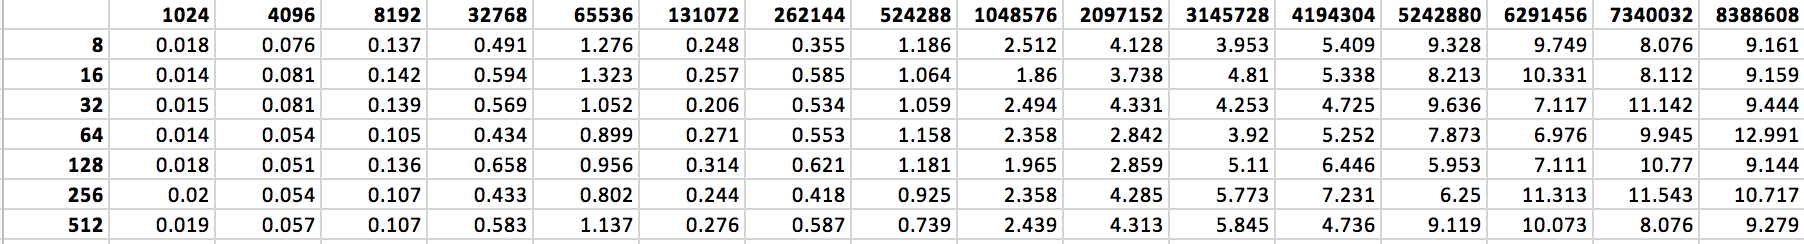
\includegraphics[width=18cm]{multTable}
				\centering
				\caption{A table of the \textit{Local Work Size} vs. \textit{Global Work Size} for the array multiplication program.
					The \textit{Local Work Size} is on the Y-axis in bold and the \textit{Global Work Size} is on the X-axis in bold. The corresponding GigaMultiplies are the values within.}
			\end{figure}
	
		\subsubsection{Array Multiplication and Add}
			\begin{figure}[H]
				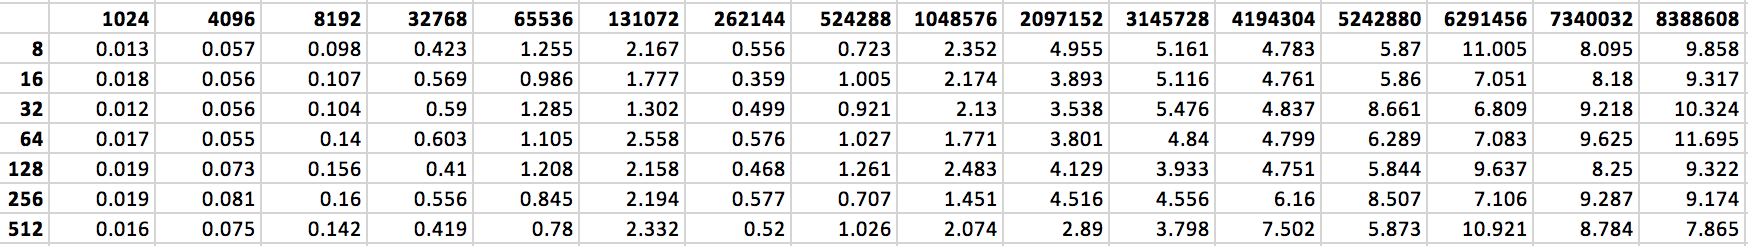
\includegraphics[width=18cm]{multAddTable}
				\centering
				\caption{A table of the \textit{Local Work Size} vs. \textit{Global Work Size} for the array multiplication and add program.
				 The \textit{Local Work Size} is on the Y-axis in bold and the \textit{Global Work Size} is on the X-axis in bold. The corresponding GigaMultiplies are the values within.}
			\end{figure}
		
		
		
		
		
	\subsection{Results Graph}
		\subsubsection{Array Multiplication}
			\begin{figure}[H]
				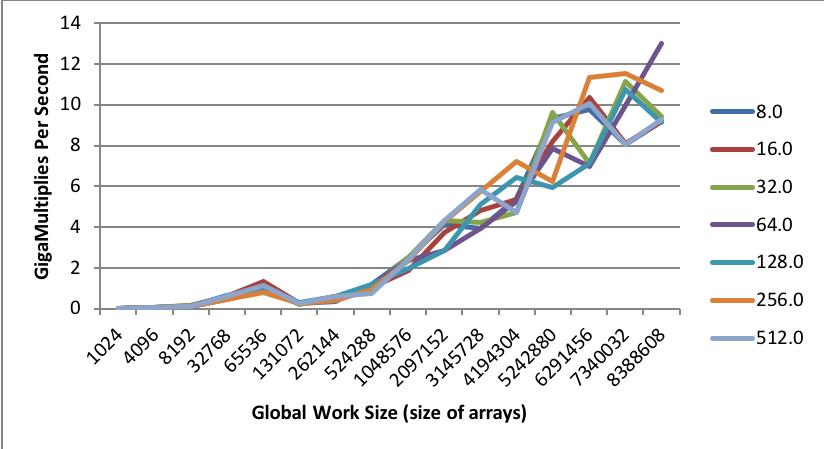
\includegraphics[width=16cm]{multGlobal}
				\centering
				\caption{A graph of the \textit{Giga Multiplies Per Second} vs. \textit{Global Work Size} for the array multiplication program.}
			\end{figure}
				
			\begin{figure}[H]
				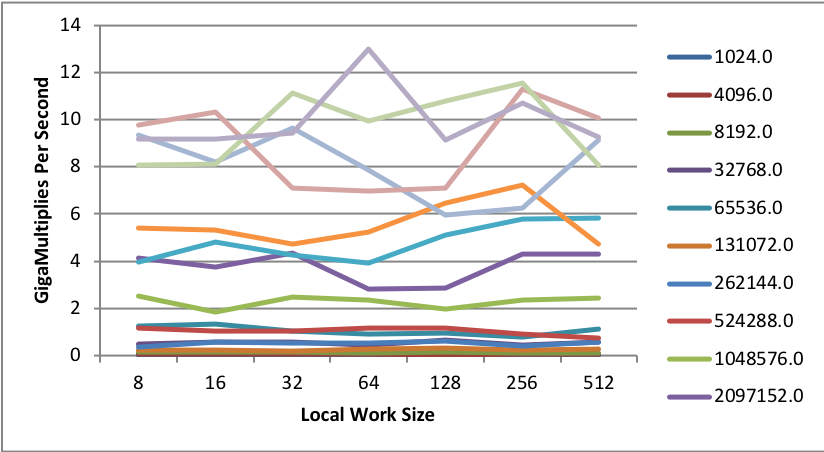
\includegraphics[width=16cm]{multLocal}
				\centering
				\caption{A graph of the \textit{Giga Multiplies Per Second} vs. \textit{Local Work Size} for the array multiplication program.}
			\end{figure}
				
				
		\subsubsection{Array Multiplication and Add}
			\begin{figure}[H]
				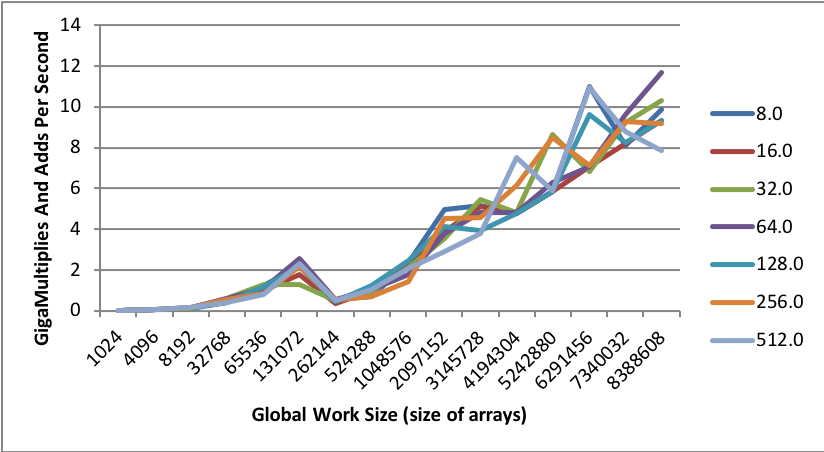
\includegraphics[width=16cm]{addGlobal}
				\centering
				\caption{A graph of the \textit{Giga Multiplies And Adds Per Second} vs. \textit{Global Work Size} for the array multiplication and add program.}
			\end{figure}
			
			\begin{figure}[H]
				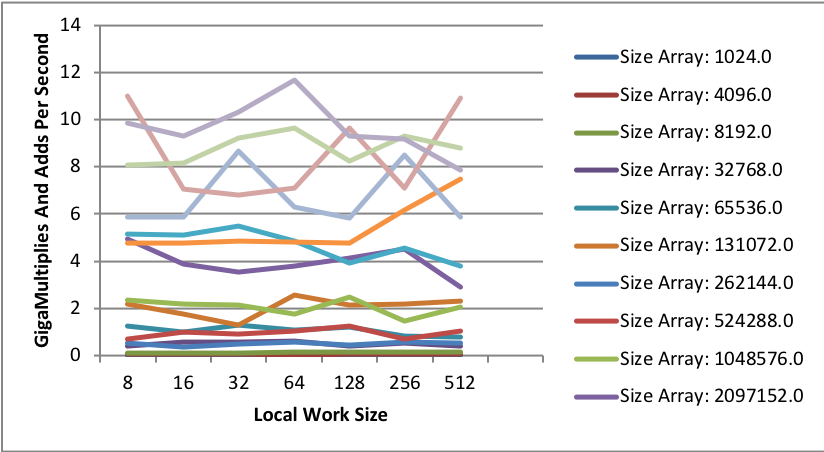
\includegraphics[width=16cm]{addLocal}
				\centering
				\caption{A graph of the \textit{Giga Multiplies And Adds Per Second} vs. \textit{Local Work Size} for the array multiplication and add program.}
			\end{figure}

			
	









	\subsection{What patterns are you seeing in the performance curves?}
		In all four of the above graphs the GigaMultiplies per second increases as the Global Work Size, size of the array, increases. 
		The Local Work Size of 64 in all of the four graphs has the highest GigaMultiplies per second.
	
	
	
	
	
	
	
	
	\subsection{Why do you think the patterns look this way?}
		I think that as the Global Work Size increases, the GigaMultiplies per second increases because GPU's work best with large data sets; that is where their power shines.
		At the bottom quarter of the graphs where the Global Work Size is between 1020 and 65536 the performance is very low. That is because the cost of the setup and preprocessing required to run on the GPU is greater than the benefit.
			
		The tests run with a Local Work Size of 64 had the highest performance. I think Local Work Sizes below 64 don't perform as well because they leave processing elements idle when they could be used.









	\subsection{What is the performance difference between doing a Multiply and doing a Multiply-Add?}
		There isn't much difference between Multiply and Multiply-add. The curves follow the same trajectory. However, on the higher Global Work Sizes Multiply is about a half GigaMultiplies per second faster (not a big difference). 
	





	
	
	
	\subsection{What does that mean for the proper use of GPU parallel computing?}
		To utilize a GPU to the best of its ability, the data set should be large; greater than 5 million elements. The right size of Local Work Size varies from task to task and GPU to GPU so it is important to do some testing. The tasks must have little user control, use regular data structures, and be parallelizeable. 








\section{Array Multiply With Reduction}
	\subsection{Results Table}
		\begin{figure}[H]
			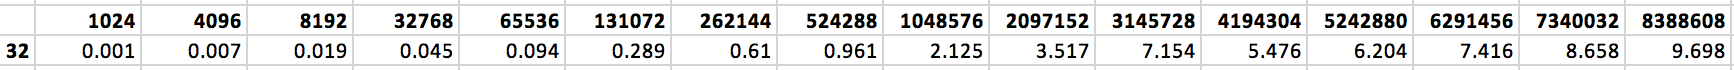
\includegraphics[width=18cm]{redTable}
			\centering
			\caption{A table of the \textit{Local Work Size} vs. \textit{Global Work Size} for the array multiplication with reduction program.
				The \textit{Local Work Size} is on the Y-axis in bold and the \textit{Global Work Size} is on the X-axis in bold. The corresponding GigaMultiplies are the values within.}
		\end{figure}
	
	
	
	
	
	\subsection{Results Graph}
		\begin{figure}[H]
			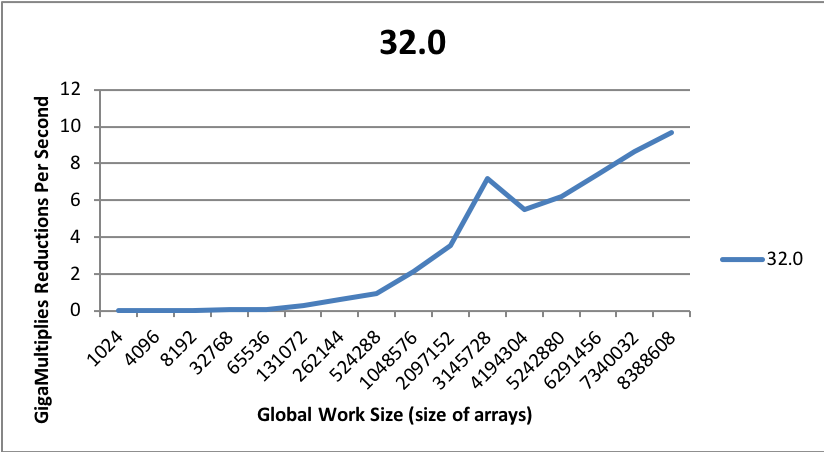
\includegraphics[width=16cm]{redGlobal}
			\centering
			\caption{A graph of the \textit{Giga Multiplies With Reductions Per Second} vs. \textit{Global Work Size} for the array multiplication with reductions program.}
		\end{figure}




	
	
	
	\subsection{What pattern are you seeing in this performance curve?}
		There isn't any performance gain until the Global Work Size is around 1048576 elements.
		The performance increases with respect to the Global Work Size.
	
	
	
	
	
	
	
	
	\subsection{Why do you think the pattern looks this way?}
		I think that as the Global Work Size increases, the GigaMultiplies per second increases because GPU's work best with large data sets.
		Global Work Sizes below 1048576 elements have a very low performance because the cost of setup and preprocessing required to run on the GPU is greater than the benefit.
	
	
	
	
	
	
	
	
	\subsection{What does that mean for the proper use of GPU parallel computing?}
		The answer is the same as above. That is, to utilize a GPU to the best of its ability, the data set should be large and easily parallizable. This can be seen by the curves increasing in performance as the Global Work Size increases.





\end{document}